\section{Related Work} % (fold)
%!TEX root = ./BPM17.tex
\label{sec:related_work}


In the following sections, the techniques and algorithms used in recent papers on predictive process monitoring that are considered as a state of the art to the problems of interest will be described. These approaches are also discussed in terms of their suitability to be used for predicting trends of activities using a-priori knowledge.

The methods are ordered in a chronological manner, each has a description of how it relates to the above-mentioned problem and a short discussion on the results and applications.

Firstly, we start off by giving a short overview of early approaches concerning predictive monitoring.
Secondly, the state of the art methods based on Complex Symbolic Sequences Encodings will be described. 
Finally, the overview of Deep learning based algorithms for predictions will be given, and it will be specified that there are no algorithms yet, that encompass the online prediction of process outcomes with A-priori knowledge.



\subsection{Early approaches}

In the early applications of business process monitoring, few mathematical models were brought to the field. The first were Petri nets~\cite{doi:10.1142/S0218126698000043}. Petri nets prove to be a very robust tool for a range of problems in process mining. They are used for conformance checking, process discovery, and process monitoring. In particular, the Petri nets were used for predictions of the business process duration~\cite{Rogge-Solti2015PBP}. 

Petri nets have few important properties such as having a formal semantics. Also, they are simple models and have graphical nature. Their properties are mathematically investigated. 

Kang and Jung~\cite{doi:10.1108/02635571111137241} propose a new approach for monitoring the progress of ongoing processes and predicting probable performances and routes. Their contribution is based on the use of Formal Concept Analysis (FCA) for monitoring business processes. They propose an alternative approach to Petri nets for visualizing the ongoing processes and predicting the future evolving (next activities) of ongoing processes by introducing concept lattice and reachability lattice. Also, to the first group of works, we can associate the work in~\cite{DBLP:journals/is/AalstSS11}. In this work, the authors present a set of approaches in which annotated transition systems, containing time information extracted from event logs, are used to: (i) check time conformance;
(ii) predict the remaining processing time of incomplete cases; (iii) recommend appropriate activities to end users working on these cases. 

In \cite{Folino}, an approach for predicting business process performances is presented. The approach is based on context-related execution scenarios discovered and modeled through state-aware performance predictors. In~\cite{Metzgeretal12}, the authors present a technique for predicting the delay between the expected and the actual arrival time of cases pertaining to a transport and logistics process. In~\cite{Senderovichetal15}, queue theory is used in order to predict possible delays in process executions.

Another group of works in the literature focuses on approaches that generate predictions and recommendations to reduce risks. For example, in~\cite{DBLP:conf/caise/ConfortiLRA13}, the authors present a technique to support process participants in making risk-informed decisions with the aim of reducing process risks. Risks are predicted by traversing decision trees generated from logs of past process executions. In~\cite{Pika}, the authors make predictions about time-related process risks by identifying and leveraging statistical indicators observable in event logs that highlight the possibility of transgressing deadlines.
In \cite{suriadi}, an approach for Root Cause Analysis (RCA) through classification algorithms is presented. These methods would suffer from low accuracy if applied in accordance of the problem stated. They usually state the probability of the process to "derail", but not predicting the full sequence of events. 


In the next section, the state of the art approaches with special process-log encoding are described.



\subsection{Prediction with Complex Symbolic Encoding for structured and unstructured content}

The second group of approaches focused on predicting the outcome (e.g., the satisfaction of a business objective) of a case can be clustered together as the methods that exploit Complex Symbolic Sequences encodings of the process log.

Complex Symbolic Sequences are introduced~\cite{Leontjeva2015}. They allow to capture a lot information about a log. Complex Symbolic Sequence is basically ordered list of vectors, where each vector is a subset of some alphabet inferred from the log.

When Complex Symbolic Sequences are used instead of Simple Symbolic Sequences (encoding that focuses solely on activity labels) for dealing with prediction problems, the complexity space of the prediction problem grows substantially. This suggests using new and more complex approaches to work with them.

Some of the base lines of working with complex symbolic sequences use index-based encodings, and index latest payload encodings mentioned in following paper~\cite{Leontjeva2015}.   

To exemplify this approach for encodings let's again take a look at the log in figure~\ref{figure:trace-example-2}. The Complex Symbolic Sequence form of this log will have following representation:

\begin{table}[h]
	\centering
	\begin{tabular}{| l | l | l | l | l | l | l | l | l |}
		\hline
		& $concept:n_{1}$ & .. & $concept:name_{3}$ & $org:resource_{1}$ & .. & $org:resource_{3}$ & $time:timestamp_{1}$ & .. \\	
		\hline
		tr1 & A\_SUBMITTED & .. & A\_DECLINED &  112 & .. & 10929 &  2011-12-12T16:06:11 & ..  \\
		tr2 &  & .. & .. & .. & .. & ..  & .. & ..  \\
		\hline
	\end{tabular}
	\caption{Example of Complex Symbolic Sequence encoding}
	\label{tab:complesymbseq_log_example}
\end{table}

Complex Symbolic Sequences allow us to encode a real log, in order to capture as much information as possible while having a structure that easily can be used with standard machine learning algorithms.

In~\cite{Leontjeva2015} the authors explore different types of encodings, called index-based encodings. They also give an alternative model called HMM-based encoding. HMM-based encoding is a direct extension to index-based, that takes into account the coefficients of the built HMM model for every possible outcome. In particular for binary classification, the log is split into two parts (according to the class) and two HMM models are built.

Basically, they look at the log, and construct a feature vector of the form:

\[g_i = (s_i^1,...,s_i^u,event_{i1},...,event_{im},h_{i1}^1,...,h_{i1}^r,...,h_{im}^1,...,h_{im}^r).\]

Where $s_i, i=\overline{1,u}$ are static features, $event_{ij}$ is an activity label event class at each position, and $h_{ik}^{j}$ are the dynamic features associated to each event. 

In~\cite{DBLP:conf/bpm/TeinemaaDMF16} the authors extends this encoding with textual, unstructured content. For this purpose they exploit methods from text mining, to extract features from textual attributes. These encodings are used with classification methods.

When Complex Symbolic Sequence encoding needs to have textual data encoded as additional parameters. A text knowledge extraction techniques, as described below are used.

First data is preprocessed is three steps: tokenized, normalized, and lemmatization is made.

Next step is encoding. The most used methods~\cite{DBLP:conf/bpm/TeinemaaDMF16} are: \textit{Bag-of-n-grams}, \textit{Naive Bayes log count ratios}, \textit{Latent Dirichlet Allocation topic modeling}, and \textit{Paragraph vector}.

After one of these methods of text encoding is chosen, the corresponding vector is appended to the index-based encoding.

This representation also has its downsides, even though it captures much more information. It is impossible to represent the complete log in this way because one needs to limit the number of events in the traces to some definite number. In our example in the table~\ref{tab:complesymbseq_log_example} the trace length was chosen to be 3. This puts a limitation on the power of this encoding.

Before mentioned approaches focus on binary classification of the traces. The problem we are solving is different as instead of predicting a binary outcome of the first $N$ events, we predict the next events. That makes the number of choices bigger (from 2 in binary classification to $K$ as a number of different possible next events). The methods described in this section, if generalized to capture the prediction of next events, would become unusable.

\subsection{Deep learning approaches} \label{deeplearning-stateoftheart}

Recently, deep learning methods became exceptionally popular in research and industry communities. Business Process Management is not an exception~\cite{quteprints96732,niek96732,evermann}. Recent papers suggest state of the art performance on the prediction of next events and time features of the current trace.

Due to the nature of the problem, i.e. sequence to sequence prediction, the recurrent neural networks are most exploited. The main motivation for this type of neural networks is currently the problems in Natural Language Processing, such as speech recognition\cite{graves2013icassp}, or translation\cite{Sutskever2014SSL29690332969173}. 

The paper by Verenich~\cite{quteprints96732}, suggests the use of Recurrent Neural Networks with sliding windows. Sliding windows is using N events to predict the next one (to predict event $k+1$,  $k..(N+k)$ events are used). The paper by Evermann\cite{evermann} proposes the use if RNN networks with LSTM cells with two hidden layers, 500 dimensions, and 20 steps. They use batches of 20 to train the RNN with back propagation. The evaluation was made on the BPI2012, BPI2013 data sets. They argue that the results with this approach are comparable to state of the art based on clustering and annotating transition system approaches. Also, the paper~\cite{evermann2} suggest developed a software suite for prediction tasks using deep learning and TensorFlow~\cite{tensorflow2015-whitepaper}.

The most recent paper by Tax~\cite{niek96732} uses RNN with LSTM cells to predict the next events. They achieve state of the art performance on most of the logs evaluated. In order to predict next event and time, they use one-hot encoding for event sequence, and few time features (such as the difference between time-stamps, time from midnight, time from the beginning of the week). Using these features they construct a vector to be fed into a recurrent neural network. They are looking for functions $f_a^1$ and $f_t^1$ that are basically the probability distributions over all possible trace continuations. Also, as they now have basically two sequences to train with, that are the sequence of events, and the sequence of time values, the paper suggests the different possible RNN architectures (As shown on figure~\ref{figure:architectureslstm}). 

\begin{figure}[!ht]
	\begin{center}  
		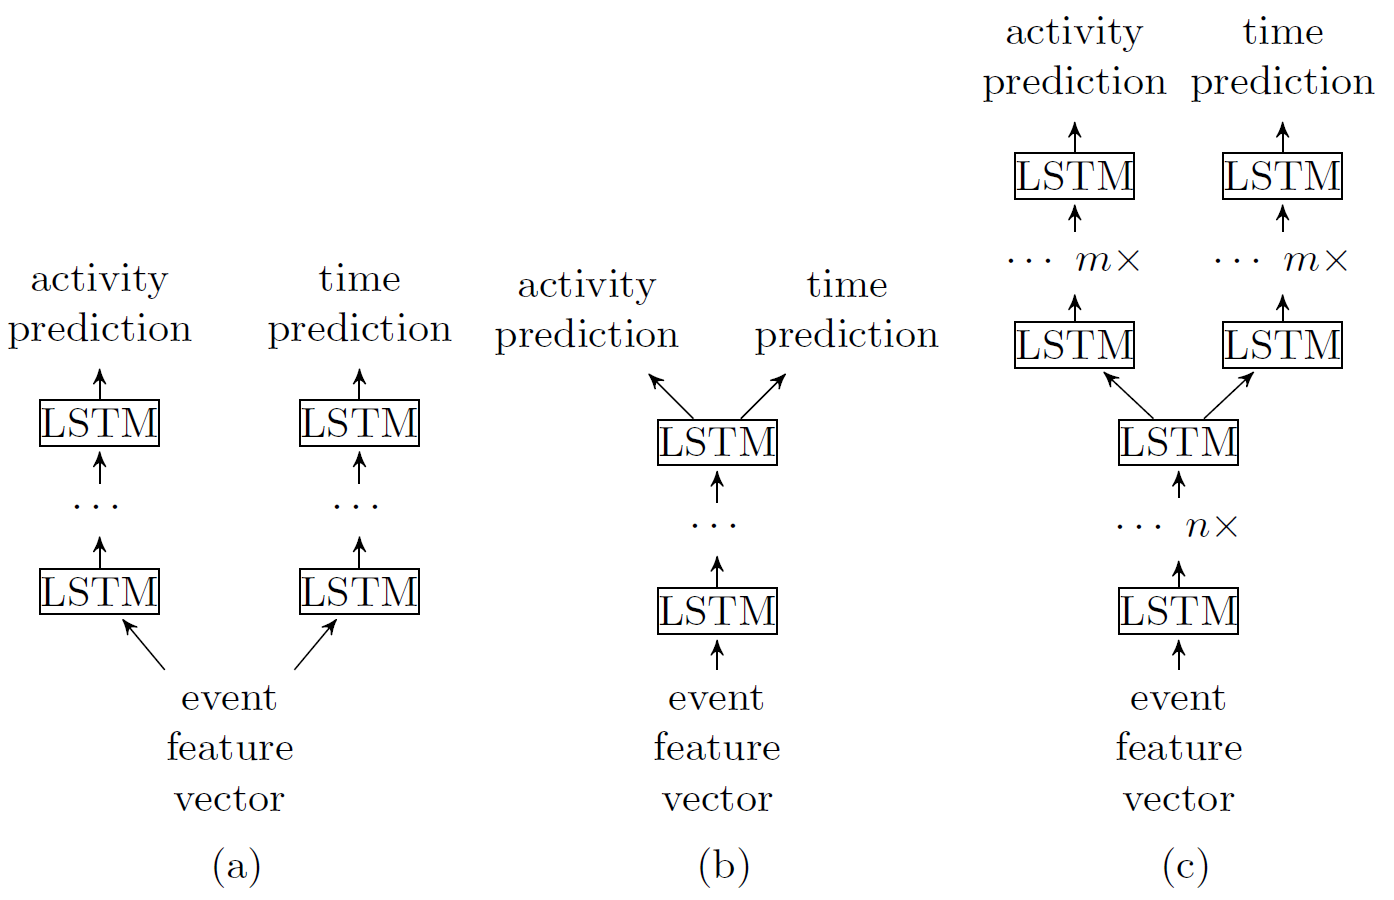
\includegraphics[width=\textwidth]{1.png}
		\caption{Possible neural network architectures \cite{niek96732}. Single task layers (a), shared multitask layers (b), or n+m shared layers (c).}
		\label{figure:architectureslstm}	
	\end{center}
\end{figure}


%The evaluation was done on many data sets, such as Helpdesk, BPI12, BPI12 with no duplicates, Environment permit. On most of them suffix (sequence of next events) prediction beats state of the art performance. It worked especially well with logs that had a lot of short traces (Helpdesk log contains average 7 event traces).

The problem investigated in this paper falls best into the problems discussed in this section i.e., into the set of very recent efforts aiming at predicting the sequence of future activities given the activities observed so far. We will exploit the state of the art architecture offered by~\cite{niek96732} in order to build a model able to leverage A-priori knowledge.

%In~\cite{Maggi:CAiSE2014} a framework is introduced, which is able to predict the fulfillment (or the violation) of a boolean predicate in a running case, by looking at: (i) the sequence of activities already performed in the case; and (ii) the data payload of the last activity of the running case. The framework, which provides accurate results at the expense of a high runtime overhead, has been enhanced in~\cite{Di-Francescomarino:2016aa} by introducing a clustering preprocessing step in which cases sharing a similar activity history are clustered together. A classifier for each cluster is trained with the data payload of the traces in the cluster. In~\cite{Leontjeva2015}, the authors compare different feature encoding approaches where traces are treated as complex symbolic sequences, that is, sequences of activities each carrying a data payload consisting of attribute-value pairs. In~\cite{DBLP:conf/bpm/TeinemaaDMF16}, the unstructured information contained in text messages exchanged during process executions has been leveraged for improving the prediction accuracy.


%~\cite{Polatoetal:2016,niek96732,evermann}.
%In~\cite{Polatoetal:2016}, Polato et al.~propose several techniques for predicting the remaining time and the sequence of future activities in an ongoing case using simple regression, regression with contextual information, and data-aware transition systems.
%
%Recently, many machine learning toolkits started leveraging the power
%of Graphical Processing Units (GPUs).  This allowed researchers and
%engineer to train their NNs in a significantly reduced amount of time:
%many complex network architectures have been trained to perform
%several task, many of them achieving remarkable performances.  Such
%innovation fostered a new interest in NNs that spread across both
%Industry and Industry.  Business Process Management is not an
%exception. \cite{quteprints96732,niek96732,evermann} Recent papers
%suggest state of the art performance on the prediction tasks for
%business process log outcomes.
%
%Due to the nature of the problem, that is the sequence to sequence prediction, the recurrent neural networks are most leveraged. The main motivation for this type of neural networks is currently the problems in Natural Language Processing, such as speech recognition\cite{graves2013icassp}, or translation\cite{Sutskever2014SSL29690332969173}.
%


%\todoincg{Fix bibentry for Niek. I would cite the technical report from which we took the data adding as a note that a version is to appear in CAISE 2017.}

%They achieve state of the art performance on most logs evaluated.
%In order to predict the next events and their timestamps, they rely on a boolean encoding of the event sequences and on few time-related features. The encoding is then used for feeding the RNN.

%In order to predict next event and time, they use one-hot encoding for event sequence, and few time features (such as difference between time-stamps, time from midnight, time from beginning of the week). Using these features they construct a vector to be fed into recurrent neural network.

%They are looking for functions $f_a^1$ and $f_t^1$ that are basically the probability distributions over all possible trace continuations.

%Also, as they now have basically two sequences to train with, that are the sequence of events, and the sequence of time values, the paper suggests the different possible RNN architectures.
%\begin{figure}[!ht]
%	\begin{center}
%		\includegraphics[width=\textwidth]{paper1233.png}
%		\caption{Possible neural network architectures \cite{niek96732}. Single task layers (a), shared multitask layers (b), or n+m shared layers (c).}
%	\end{center}
%\end{figure}

%The evaluation was done on many data sets, such as Helpdesk, BPI12, BPI12 with no duplicates, Environment permit. On most of them suffix (sequence of next events) prediction beats state of the art performance. It worked especially well with logs that had a lot of short traces (Helpdesk log contains average 7 event traces).
%%% Local Variables:
%%% mode: latex
%%% TeX-master: "BPM17"
%%% End:
